\StartPlate{V03}{A balanced central product}{The shared center is identified once, while the orthogonal packet factors remain.}
\begin{center}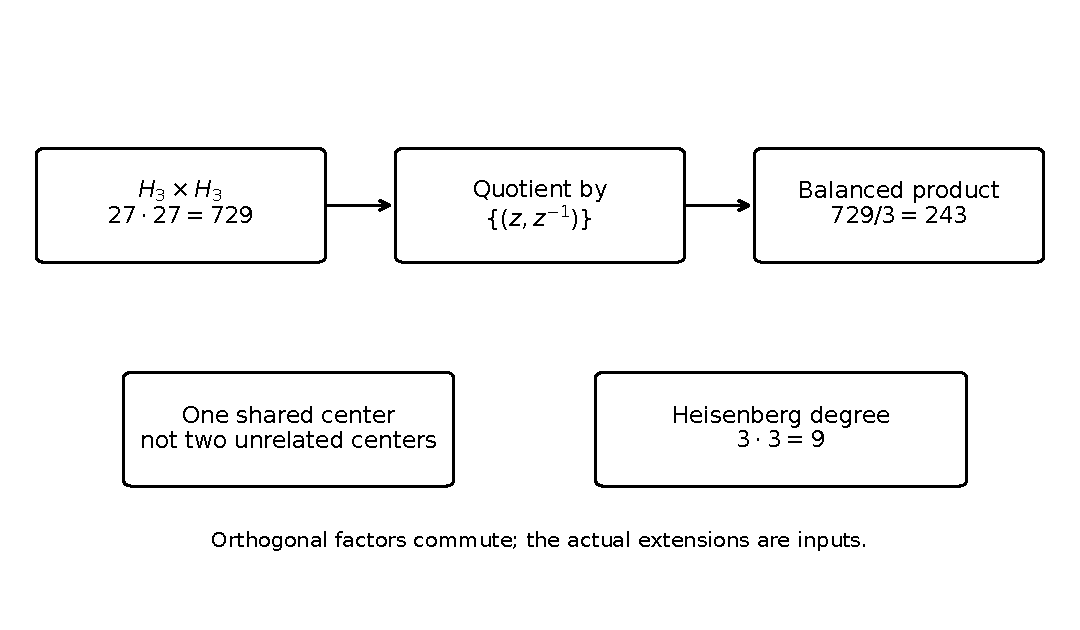
\includegraphics[width=\linewidth]{figures/V03.pdf}\end{center}
Take two Heisenberg groups of order $3^3=27$. Their direct product has order $729$. Quotient by the central subgroup $\{(z,z^{-1})\}$ of order three. The balanced central product has order $3^5=243$, with a four-dimensional quotient over $\F_3$ and one common center.
\[
(H_3\times H_3)/\{(z,z^{-1})\}
\quad\text{has Heisenberg degree}\quad 3^2=9.
\]
The figure's order calculation is checked by enumerating every fibre of the multiplication model. Each fibre has exactly three elements. The representation degree agrees with the tensor product of two degree-three Heisenberg representations whose central characters match.

The general argument requires the actual factor extensions and commutation between distinct factors. A list of break labels does not supply either condition. Once those conditions hold, the balanced product removes the proposed extra mixed extension ambiguity. It does not construct an arithmetic host or identify independently fixed lifts.
\vfill\PlateSource{Exact finite model}{Part I, Section 3}{8}
